\hypertarget{LinearStatistic_8c}{
\section{LinearStatistic.c File Reference}
\label{LinearStatistic_8c}\index{LinearStatistic.c@{LinearStatistic.c}}
}
{\tt \#include \char`\"{}coin\_\-common.h\char`\"{}}\par


Include dependency graph for LinearStatistic.c:\nopagebreak
\begin{figure}[H]
\begin{center}
\leavevmode
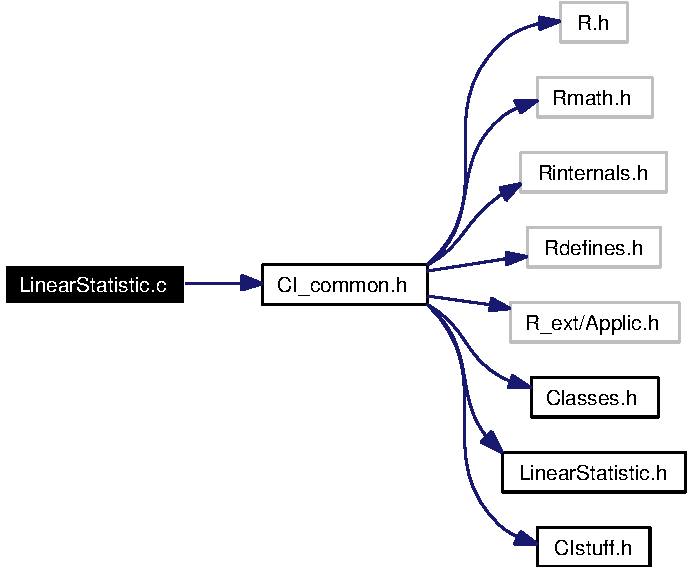
\includegraphics[width=350pt]{LinearStatistic_8c__incl}
\end{center}
\end{figure}
\subsection*{Functions}
\begin{CompactItemize}
\item 
void \hyperlink{LinearStatistic_8c_12e882779ecd0445c3a0dd9ac85dfeee}{C\_\-kronecker} (const double $\ast$A, const int m, const int n, const double $\ast$B, const int r, const int s, double $\ast$ans)
\item 
SEXP \hyperlink{LinearStatistic_8c_95f5ed4c75d42e2e98ed09c9c9d48ff5}{R\_\-kronecker} (SEXP A, SEXP B)
\item 
void \hyperlink{LinearStatistic_8c_e2f62abe13ee5b625141b5d4a496d832}{C\_\-ExpectCovarInfluence} (const double $\ast$y, const int q, const double $\ast$weights, const int n, SEXP ans)
\item 
SEXP \hyperlink{LinearStatistic_8c_6216ea560644c08002fb32756ae67dcc}{R\_\-ExpectCovarInfluence} (SEXP y, SEXP weights)
\item 
void \hyperlink{LinearStatistic_8c_94a0805ea258af79d426c095feee399a}{C\_\-ExpectCovarLinearStatistic} (const double $\ast$x, const int p, const double $\ast$y, const int q, const double $\ast$weights, const int n, const SEXP expcovinf, SEXP ans)
\item 
SEXP \hyperlink{LinearStatistic_8c_58fff8082d3ab197994a21a10c422353}{R\_\-ExpectCovarLinearStatistic} (SEXP x, SEXP y, SEXP weights, SEXP expcovinf)
\item 
void \hyperlink{LinearStatistic_8c_aefa2a9406bb30b323715e3db41da637}{C\_\-LinearStatistic} (const double $\ast$x, const int p, const double $\ast$y, const int q, const double $\ast$weights, const int n, double $\ast$ans)
\item 
SEXP \hyperlink{LinearStatistic_8c_732bfc8e1797d8953482aa31f9b43e5f}{R\_\-LinearStatistic} (SEXP x, SEXP y, SEXP weights)
\item 
void \hyperlink{LinearStatistic_8c_a34b0f12fac36231a105d6dc903bfe89}{C\_\-PermutedLinearStatistic} (const double $\ast$x, const int p, const double $\ast$y, const int q, const int n, const int nperm, const int $\ast$indx, const int $\ast$perm, double $\ast$ans)
\item 
SEXP \hyperlink{LinearStatistic_8c_be383bcae17e8b3a1d5740ec16a9817a}{R\_\-PermutedLinearStatistic} (SEXP x, SEXP y, SEXP indx, SEXP perm)
\end{CompactItemize}


\subsection{Detailed Description}
Linear statistics for conditional inference

\begin{Desc}
\item[Author:]\begin{Desc}
\item[Author]\end{Desc}
\end{Desc}
\begin{Desc}
\item[Date:]\begin{Desc}
\item[Date]\end{Desc}
\end{Desc}


Definition in file \hyperlink{LinearStatistic_8c-source}{LinearStatistic.c}.

\subsection{Function Documentation}
\hypertarget{LinearStatistic_8c_e2f62abe13ee5b625141b5d4a496d832}{
\index{LinearStatistic.c@{LinearStatistic.c}!C_ExpectCovarInfluence@{C\_\-ExpectCovarInfluence}}
\index{C_ExpectCovarInfluence@{C\_\-ExpectCovarInfluence}!LinearStatistic.c@{LinearStatistic.c}}
\subsubsection{\setlength{\rightskip}{0pt plus 5cm}void C\_\-ExpectCovarInfluence (const double $\ast$ {\em y}, const int {\em q}, const double $\ast$ {\em weights}, const int {\em n}, SEXP {\em ans})}}
\label{LinearStatistic_8c_e2f62abe13ee5b625141b5d4a496d832}


Conditional expectation and covariance of the influence function\par
 \begin{Desc}
\item[Parameters:]
\begin{description}
\item[{\em y}]values of the influence function \item[{\em q}]dimension of the influence function \item[{\em weights}]case weights \item[{\em n}]number of observations \item[{\em ans}]return value; an object of class `ExpectCovarInfluence' \end{description}
\end{Desc}


Definition at line 80 of file LinearStatistic.c.

References coin\_\-covarianceSym, coin\_\-expectationSym, and coin\_\-sumweightsSym.

Referenced by R\_\-ExpectCovarInfluence().\hypertarget{LinearStatistic_8c_94a0805ea258af79d426c095feee399a}{
\index{LinearStatistic.c@{LinearStatistic.c}!C_ExpectCovarLinearStatistic@{C\_\-ExpectCovarLinearStatistic}}
\index{C_ExpectCovarLinearStatistic@{C\_\-ExpectCovarLinearStatistic}!LinearStatistic.c@{LinearStatistic.c}}
\subsubsection{\setlength{\rightskip}{0pt plus 5cm}void C\_\-ExpectCovarLinearStatistic (const double $\ast$ {\em x}, const int {\em p}, const double $\ast$ {\em y}, const int {\em q}, const double $\ast$ {\em weights}, const int {\em n}, const SEXP {\em expcovinf}, SEXP {\em ans})}}
\label{LinearStatistic_8c_94a0805ea258af79d426c095feee399a}


Conditional expectation and covariance of the a linear statistic\par
 \begin{Desc}
\item[Parameters:]
\begin{description}
\item[{\em x}]values of the transformation \item[{\em p}]dimension of the transformation \item[{\em y}]values of the influence function \item[{\em q}]dimension of the influence function \item[{\em weights}]case weights \item[{\em n}]number of observations \item[{\em expcovinf}]an object of class `ExpectCovarInfluence' \item[{\em ans}]return value; an object of class `ExpectCovar' \end{description}
\end{Desc}


Definition at line 192 of file LinearStatistic.c.

References C\_\-kronecker(), coin\_\-covarianceSym, coin\_\-expectationSym, and coin\_\-sumweightsSym.

Referenced by R\_\-ExpectCovarLinearStatistic().

Here is the call graph for this function:\nopagebreak
\begin{figure}[H]
\begin{center}
\leavevmode
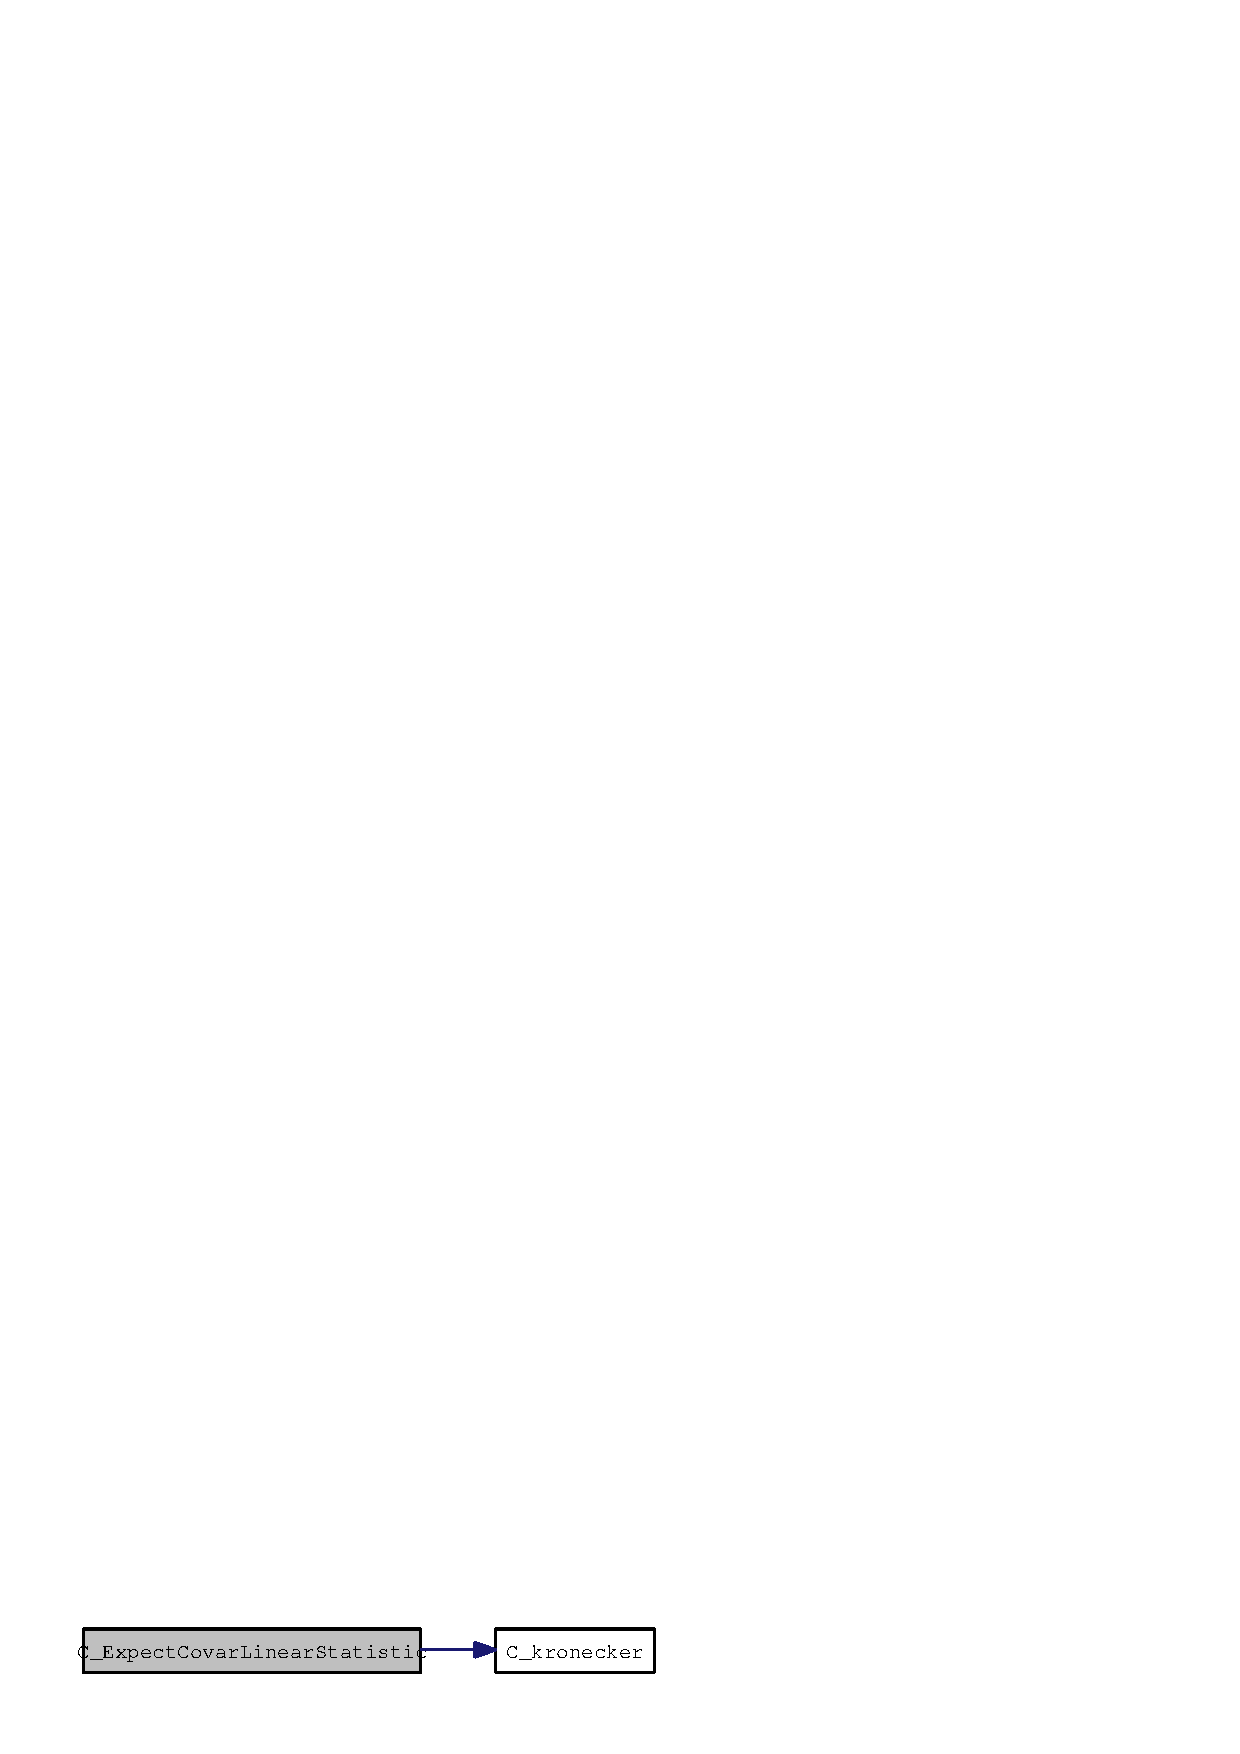
\includegraphics[width=159pt]{LinearStatistic_8c_94a0805ea258af79d426c095feee399a_cgraph}
\end{center}
\end{figure}
\hypertarget{LinearStatistic_8c_12e882779ecd0445c3a0dd9ac85dfeee}{
\index{LinearStatistic.c@{LinearStatistic.c}!C_kronecker@{C\_\-kronecker}}
\index{C_kronecker@{C\_\-kronecker}!LinearStatistic.c@{LinearStatistic.c}}
\subsubsection{\setlength{\rightskip}{0pt plus 5cm}void C\_\-kronecker (const double $\ast$ {\em A}, const int {\em m}, const int {\em n}, const double $\ast$ {\em B}, const int {\em r}, const int {\em s}, double $\ast$ {\em ans})}}
\label{LinearStatistic_8c_12e882779ecd0445c3a0dd9ac85dfeee}


Computes the Kronecker product of two matrices\par
 \begin{Desc}
\item[Parameters:]
\begin{description}
\item[{\em A}]matrix \item[{\em m}]nrow(A) \item[{\em n}]ncol(A) \item[{\em B}]matrix \item[{\em r}]nrow(B) \item[{\em s}]ncol(B) \item[{\em ans}]return value; a pointer to a REALSXP-vector of length (mr x ns) \end{description}
\end{Desc}


Definition at line 22 of file LinearStatistic.c.

Referenced by C\_\-ExpectCovarLinearStatistic(), and R\_\-kronecker().\hypertarget{LinearStatistic_8c_aefa2a9406bb30b323715e3db41da637}{
\index{LinearStatistic.c@{LinearStatistic.c}!C_LinearStatistic@{C\_\-LinearStatistic}}
\index{C_LinearStatistic@{C\_\-LinearStatistic}!LinearStatistic.c@{LinearStatistic.c}}
\subsubsection{\setlength{\rightskip}{0pt plus 5cm}void C\_\-LinearStatistic (const double $\ast$ {\em x}, const int {\em p}, const double $\ast$ {\em y}, const int {\em q}, const double $\ast$ {\em weights}, const int {\em n}, double $\ast$ {\em ans})}}
\label{LinearStatistic_8c_aefa2a9406bb30b323715e3db41da637}


Computes the linear statistic, formula (1) in the paper\par
 \begin{Desc}
\item[Parameters:]
\begin{description}
\item[{\em x}]values of the transformation \item[{\em p}]dimension of the transformation \item[{\em y}]values of the influence function \item[{\em q}]dimension of the influence function \item[{\em weights}]case weights \item[{\em n}]number of observations \item[{\em ans}]return value; a pointer to a REALSXP-vector of length pq \end{description}
\end{Desc}


Definition at line 327 of file LinearStatistic.c.

Referenced by R\_\-LinearStatistic().\hypertarget{LinearStatistic_8c_a34b0f12fac36231a105d6dc903bfe89}{
\index{LinearStatistic.c@{LinearStatistic.c}!C_PermutedLinearStatistic@{C\_\-PermutedLinearStatistic}}
\index{C_PermutedLinearStatistic@{C\_\-PermutedLinearStatistic}!LinearStatistic.c@{LinearStatistic.c}}
\subsubsection{\setlength{\rightskip}{0pt plus 5cm}void C\_\-PermutedLinearStatistic (const double $\ast$ {\em x}, const int {\em p}, const double $\ast$ {\em y}, const int {\em q}, const int {\em n}, const int {\em nperm}, const int $\ast$ {\em indx}, const int $\ast$ {\em perm}, double $\ast$ {\em ans})}}
\label{LinearStatistic_8c_a34b0f12fac36231a105d6dc903bfe89}


Linear Statistic with permuted indices\par
 \begin{Desc}
\item[Parameters:]
\begin{description}
\item[{\em x}]values of the transformation \item[{\em p}]dimension of the transformation \item[{\em y}]values of the influence function \item[{\em q}]dimension of the influence function \item[{\em n}]number of observations \item[{\em nperm}]number of permutations \item[{\em indx}]indices for the x-part \item[{\em perm}](permuted) indices for the y-part \item[{\em ans}]return value; a pointer to a REALSXP-vector of length pq \end{description}
\end{Desc}


Definition at line 409 of file LinearStatistic.c.

Referenced by R\_\-MonteCarloIndependenceTest(), and R\_\-PermutedLinearStatistic().\hypertarget{LinearStatistic_8c_6216ea560644c08002fb32756ae67dcc}{
\index{LinearStatistic.c@{LinearStatistic.c}!R_ExpectCovarInfluence@{R\_\-ExpectCovarInfluence}}
\index{R_ExpectCovarInfluence@{R\_\-ExpectCovarInfluence}!LinearStatistic.c@{LinearStatistic.c}}
\subsubsection{\setlength{\rightskip}{0pt plus 5cm}SEXP R\_\-ExpectCovarInfluence (SEXP {\em y}, SEXP {\em weights})}}
\label{LinearStatistic_8c_6216ea560644c08002fb32756ae67dcc}


R-interface to C\_\-ExpectCovarInfluence\par
 \begin{Desc}
\item[Parameters:]
\begin{description}
\item[{\em y}]values of the influence function \item[{\em weights}]case weights \end{description}
\end{Desc}


Definition at line 150 of file LinearStatistic.c.

References C\_\-ExpectCovarInfluence(), coin\_\-covarianceSym, coin\_\-expectationSym, coin\_\-sumweightsSym, ncol(), and nrow().

Here is the call graph for this function:\nopagebreak
\begin{figure}[H]
\begin{center}
\leavevmode
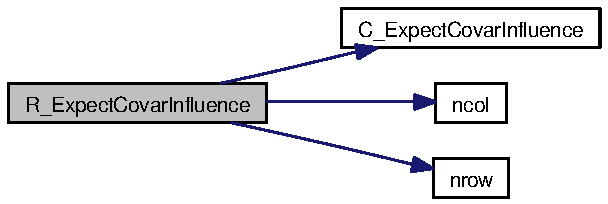
\includegraphics[width=177pt]{LinearStatistic_8c_6216ea560644c08002fb32756ae67dcc_cgraph}
\end{center}
\end{figure}
\hypertarget{LinearStatistic_8c_58fff8082d3ab197994a21a10c422353}{
\index{LinearStatistic.c@{LinearStatistic.c}!R_ExpectCovarLinearStatistic@{R\_\-ExpectCovarLinearStatistic}}
\index{R_ExpectCovarLinearStatistic@{R\_\-ExpectCovarLinearStatistic}!LinearStatistic.c@{LinearStatistic.c}}
\subsubsection{\setlength{\rightskip}{0pt plus 5cm}SEXP R\_\-ExpectCovarLinearStatistic (SEXP {\em x}, SEXP {\em y}, SEXP {\em weights}, SEXP {\em expcovinf})}}
\label{LinearStatistic_8c_58fff8082d3ab197994a21a10c422353}


R-interface to C\_\-ExpectCovarLinearStatistic\par
 \begin{Desc}
\item[Parameters:]
\begin{description}
\item[{\em x}]values of the transformation \item[{\em y}]values of the influence function \item[{\em weights}]case weights \item[{\em expcovinf}]an object of class `ExpectCovarInfluence' \end{description}
\end{Desc}


Definition at line 285 of file LinearStatistic.c.

References C\_\-ExpectCovarLinearStatistic(), coin\_\-covarianceSym, coin\_\-expectationSym, ncol(), and nrow().

Here is the call graph for this function:\nopagebreak
\begin{figure}[H]
\begin{center}
\leavevmode
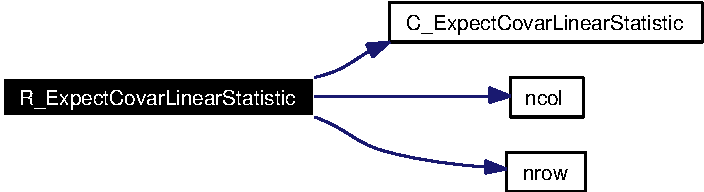
\includegraphics[width=258pt]{LinearStatistic_8c_58fff8082d3ab197994a21a10c422353_cgraph}
\end{center}
\end{figure}
\hypertarget{LinearStatistic_8c_95f5ed4c75d42e2e98ed09c9c9d48ff5}{
\index{LinearStatistic.c@{LinearStatistic.c}!R_kronecker@{R\_\-kronecker}}
\index{R_kronecker@{R\_\-kronecker}!LinearStatistic.c@{LinearStatistic.c}}
\subsubsection{\setlength{\rightskip}{0pt plus 5cm}SEXP R\_\-kronecker (SEXP {\em A}, SEXP {\em B})}}
\label{LinearStatistic_8c_95f5ed4c75d42e2e98ed09c9c9d48ff5}


R-interface to C\_\-kronecker\par
 \begin{Desc}
\item[Parameters:]
\begin{description}
\item[{\em A}]matrix \item[{\em B}]matrix \end{description}
\end{Desc}


Definition at line 51 of file LinearStatistic.c.

References C\_\-kronecker(), ncol(), and nrow().

Here is the call graph for this function:\nopagebreak
\begin{figure}[H]
\begin{center}
\leavevmode
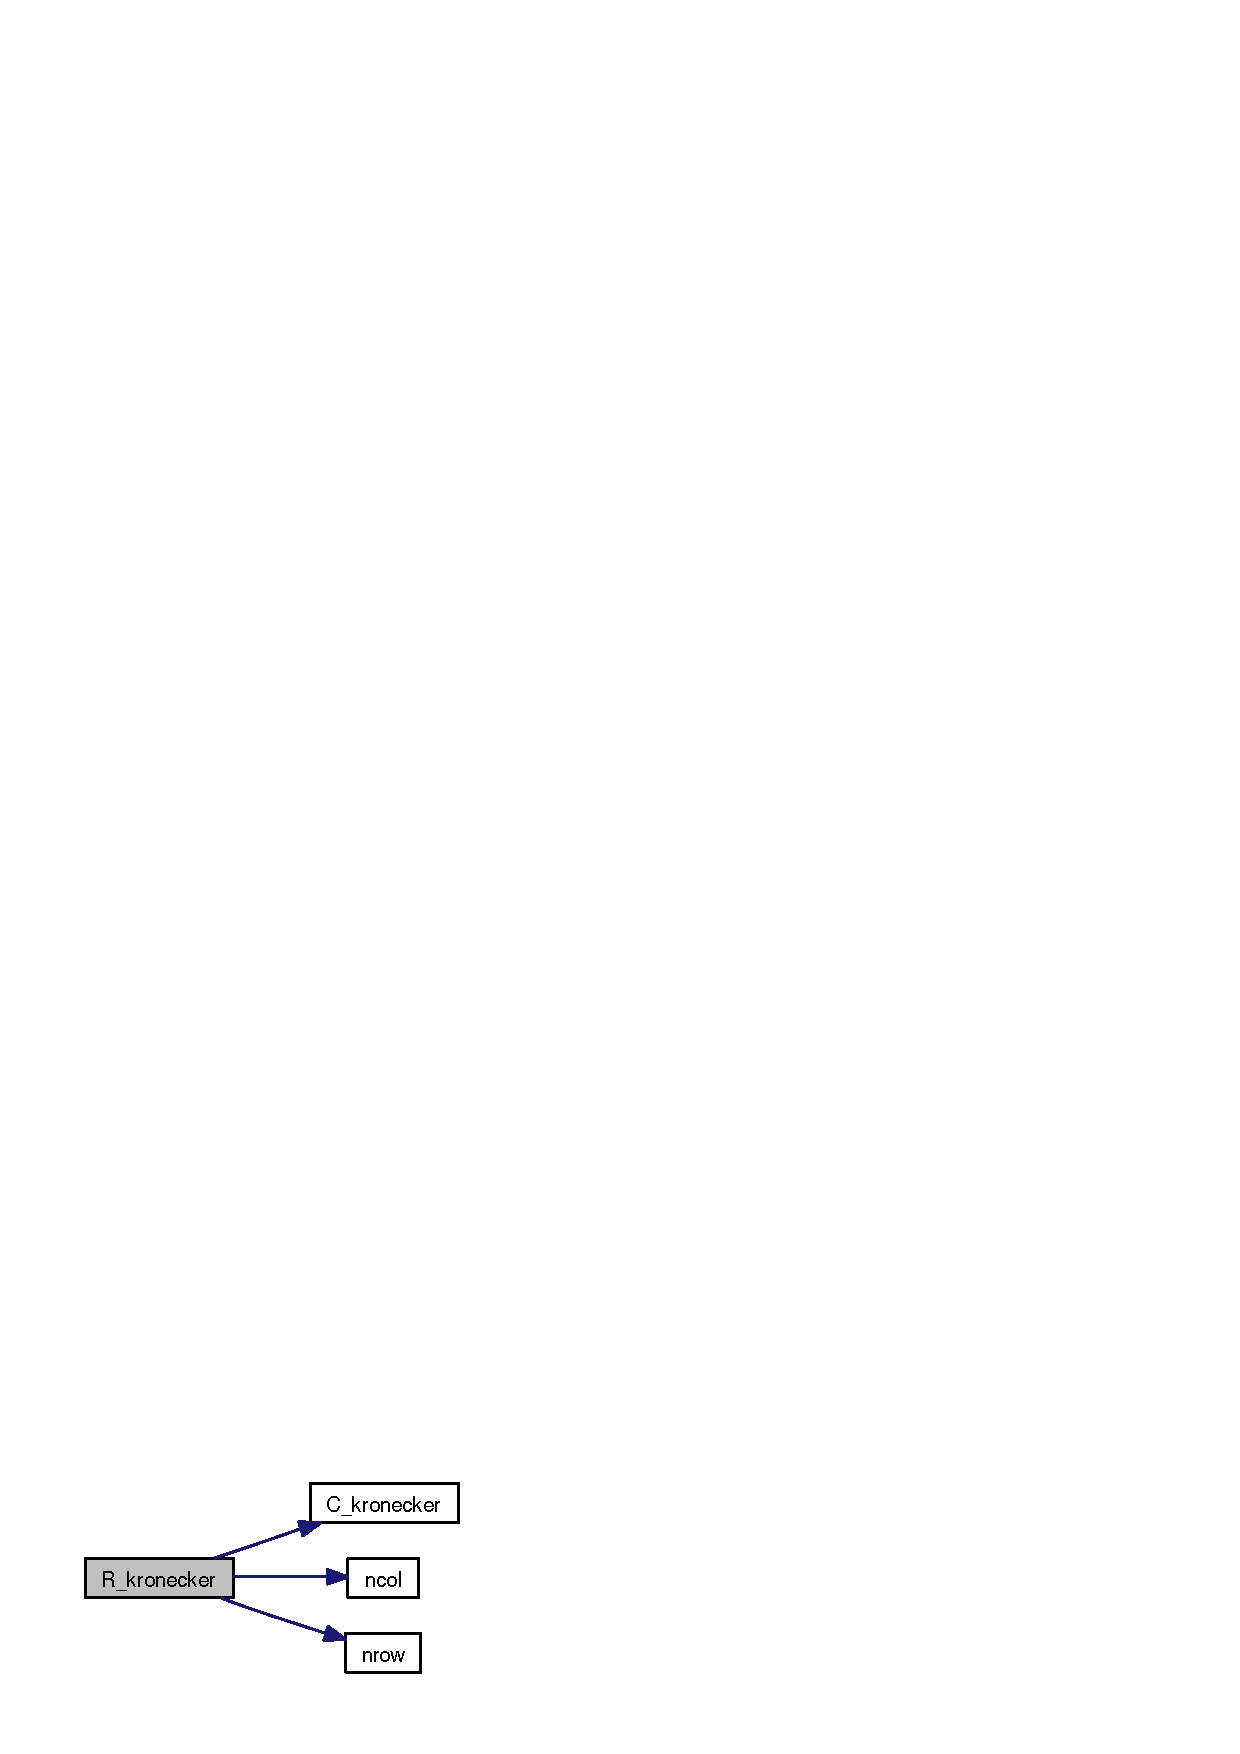
\includegraphics[width=116pt]{LinearStatistic_8c_95f5ed4c75d42e2e98ed09c9c9d48ff5_cgraph}
\end{center}
\end{figure}
\hypertarget{LinearStatistic_8c_732bfc8e1797d8953482aa31f9b43e5f}{
\index{LinearStatistic.c@{LinearStatistic.c}!R_LinearStatistic@{R\_\-LinearStatistic}}
\index{R_LinearStatistic@{R\_\-LinearStatistic}!LinearStatistic.c@{LinearStatistic.c}}
\subsubsection{\setlength{\rightskip}{0pt plus 5cm}SEXP R\_\-LinearStatistic (SEXP {\em x}, SEXP {\em y}, SEXP {\em weights})}}
\label{LinearStatistic_8c_732bfc8e1797d8953482aa31f9b43e5f}


R-interface to C\_\-LinearStatistic \par
 \begin{Desc}
\item[Parameters:]
\begin{description}
\item[{\em x}]values of the transformation \item[{\em y}]values of the influence function \item[{\em weights}]case weights \end{description}
\end{Desc}


Definition at line 363 of file LinearStatistic.c.

References C\_\-LinearStatistic(), ncol(), and nrow().

Here is the call graph for this function:\nopagebreak
\begin{figure}[H]
\begin{center}
\leavevmode
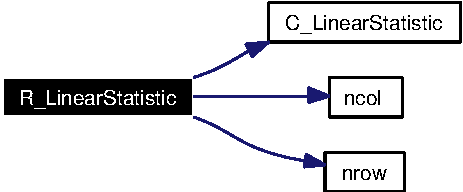
\includegraphics[width=138pt]{LinearStatistic_8c_732bfc8e1797d8953482aa31f9b43e5f_cgraph}
\end{center}
\end{figure}
\hypertarget{LinearStatistic_8c_be383bcae17e8b3a1d5740ec16a9817a}{
\index{LinearStatistic.c@{LinearStatistic.c}!R_PermutedLinearStatistic@{R\_\-PermutedLinearStatistic}}
\index{R_PermutedLinearStatistic@{R\_\-PermutedLinearStatistic}!LinearStatistic.c@{LinearStatistic.c}}
\subsubsection{\setlength{\rightskip}{0pt plus 5cm}SEXP R\_\-PermutedLinearStatistic (SEXP {\em x}, SEXP {\em y}, SEXP {\em indx}, SEXP {\em perm})}}
\label{LinearStatistic_8c_be383bcae17e8b3a1d5740ec16a9817a}


Linear Statistic with permuted indices\par
 \begin{Desc}
\item[Parameters:]
\begin{description}
\item[{\em x}]values of the transformation \item[{\em y}]values of the influence function \item[{\em indx}]indices for the x-part \item[{\em perm}](permuted) indices for the y-part \end{description}
\end{Desc}


Definition at line 442 of file LinearStatistic.c.

References C\_\-PermutedLinearStatistic(), ncol(), and nrow().

Here is the call graph for this function:\nopagebreak
\begin{figure}[H]
\begin{center}
\leavevmode
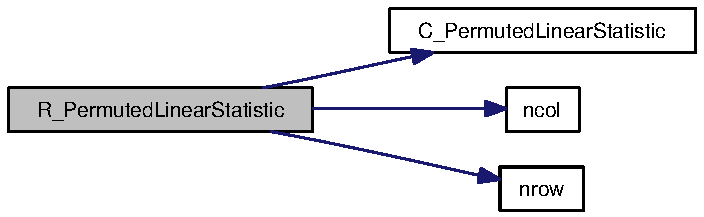
\includegraphics[width=187pt]{LinearStatistic_8c_be383bcae17e8b3a1d5740ec16a9817a_cgraph}
\end{center}
\end{figure}
